\documentclass{extbook}
\usepackage[papersize={8.5in,11in},top=1in,bottom=1in]{geometry}
\RequirePackage{fix-cm}
\usepackage[T1]{fontenc}
\usepackage{lmodern}
\usepackage{fullpage}
\usepackage{titlesec}
\usepackage{parskip}
\usepackage{float}
\usepackage{url}
\usepackage{hyperref}
\usepackage{graphicx}
\usepackage{tcolorbox}
\usepackage{tabularx}
\usepackage{xcolor}
\usepackage{titlesec}
\usepackage{amsmath}
\usepackage{tcolorbox}
\usepackage{tabularx}

\renewcommand{\contentsname}{Contenido}
\renewcommand{\figurename}{Figura}
%\renewcommand{\listtablename}{Lista de tablas}
\renewcommand{\listfigurename}{Lista de figuras}
\usepackage[fontsize=13.5pt]{fontsize}
\setlength{\parindent}{0pt}

\titleformat{\chapter}[display]
  {\bfseries\huge} % Estilo del título
  {\hfill\Large} % Alineación a la derecha
  {3ex} % Espaciado entre el número del capítulo y el título
  {\vspace{-5cm}\titlerule\vspace{1.5ex}\hfill} % Regla arriba y alineación del título a la derecha
  [\vspace{1ex}\titlerule] % Regla debajo del título


  \makeatletter
  \patchcmd{\chapter}
    {\if@openright\cleardoublepage\else\clearpage\fi}
    {\clearpage}
    {}{}
  \makeatother

  \definecolor{codegreen}{rgb}{0,0.6,0}
  \definecolor{codegray}{rgb}{0.5,0.5,0.5}
  \definecolor{codepurple}{rgb}{0.58,0,0.82}
  \definecolor{backcolour}{rgb}{0.95,0.95,0.92}

\begin{document}
\begin{titlepage}
  \begin{center}
      {\huge \textbf{Universidad Tecnológica de Panamá}}\\
      \vspace{3mm}
      {\Large \textbf{Centro Regional De Veraguas}}

      \begin{figure}[H]
          \centering
          
\includegraphics[scale = 0.07]{Imagenes/UTP/utp.png}
          
\includegraphics[scale = 0.58]{Imagenes/UTP/fisc.png}
      \end{figure}
      {\Large \textbf{Facultad de Ingeniería de Sistemas Computacionales}}\\
      \vspace{5mm}
      
      {\Large \textbf{Curso: Base de Datos II}}\medskip
      
      {\Large \textbf{Profesor: Carlos Herrera}}

      \rule{\linewidth}{0.75mm}\\
          {\Large \textsc{Laboratorio 4}} 
      \rule{\linewidth}{0.75mm}\medskip

      {\Large \textbf{Estudiante}}\\
      \vspace{5mm}
      {\Large \textbf{Arland Barrera}}
      \vfill
      {\Huge \textbf{2024}}

  \end{center}
\end{titlepage}
\tableofcontents
\listoffigures
%\listoftables para lista de tablas
\chapter{Desarrollo}
\section{Problemas resueltos}
\subsection{Problema resuelto 1}

\begin{figure}[H]
  \centering
  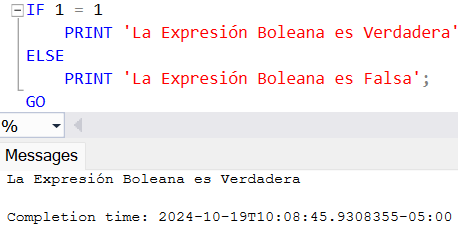
\includegraphics{Imagenes/probs_resueltos/pr1.png}
  \caption{Problema resuelto 1}
\end{figure}

\subsection{Problema resuelto 2}

\begin{figure}[H]
  \centering
  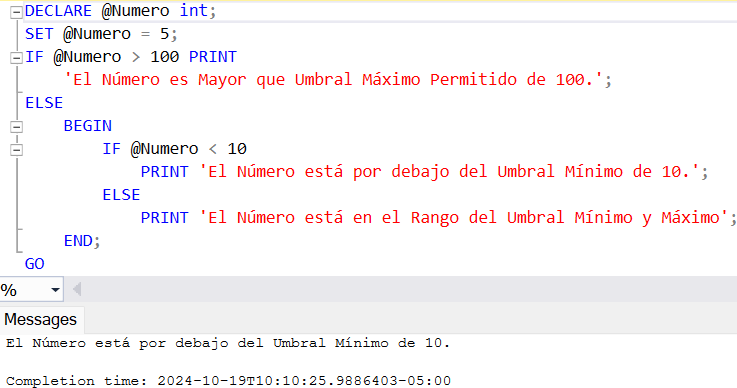
\includegraphics[scale = 0.5]{Imagenes/probs_resueltos/pr2.png}
  \caption{Problema resuelto 2}
\end{figure}

\subsection{Problema resuelto 3}

\begin{figure}[H]
  \centering
  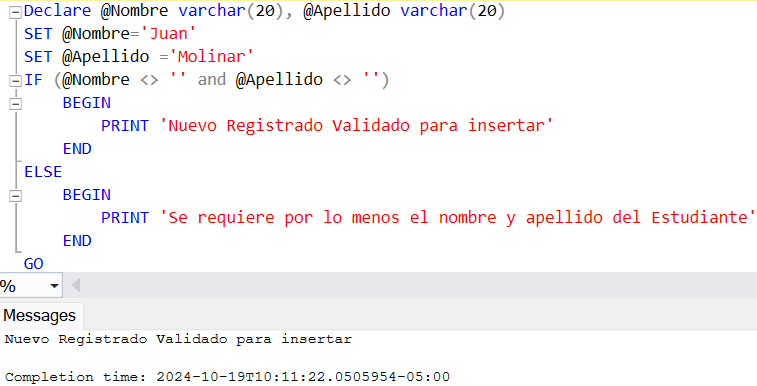
\includegraphics[scale = 0.5]{Imagenes/probs_resueltos/pr3.png}
  \caption{Problema resuelto 3}
\end{figure}

\subsection{Problema resuelto 4}

\begin{figure}[H]
  \centering
  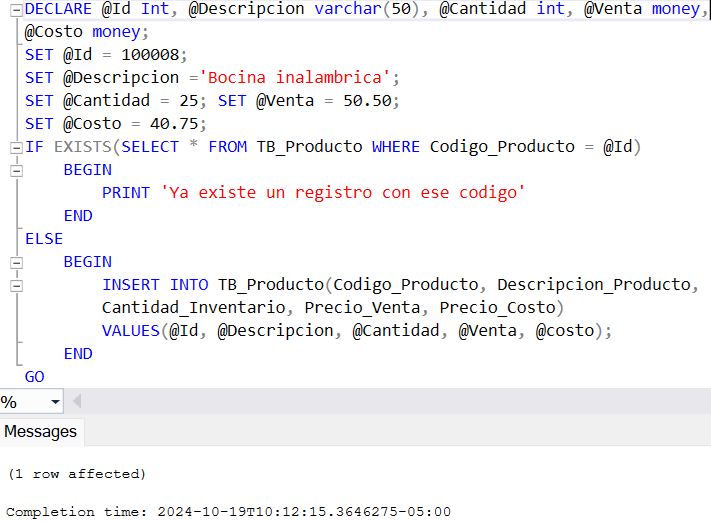
\includegraphics[scale = 0.5]{Imagenes/probs_resueltos/pr4.png}
  \caption{Problema resuelto 4}
\end{figure}

\subsection{Problema resuelto 5}

\begin{figure}[H]
  \centering
  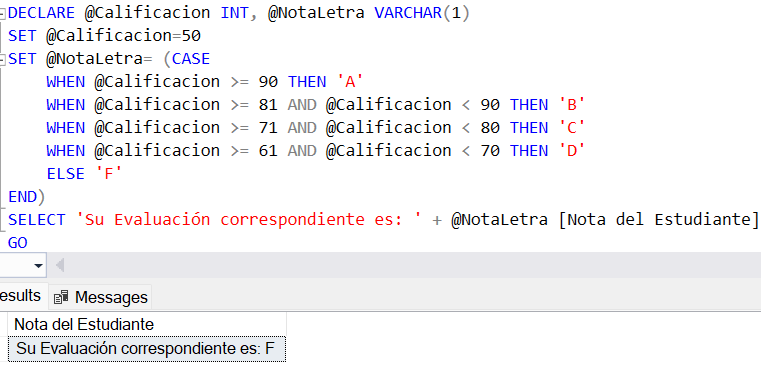
\includegraphics[scale = 0.5]{Imagenes/probs_resueltos/pr5.png}
  \caption{Problema resuelto 5}
\end{figure}

\subsection{Problema resuelto 6}

\begin{figure}[H]
  \centering
  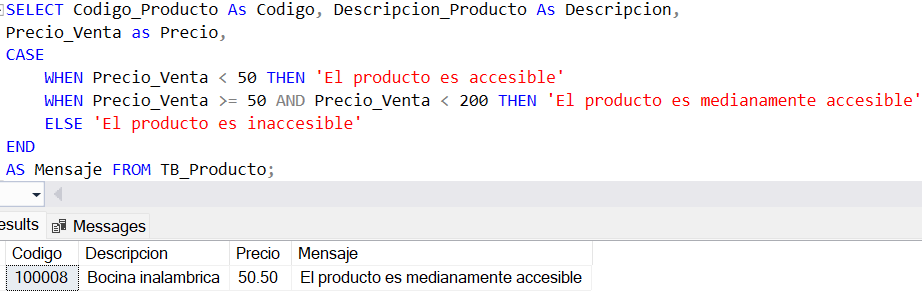
\includegraphics[scale = 0.5]{Imagenes/probs_resueltos/pr6.png}
  \caption{Problema resuelto 6}
\end{figure}

\subsection{Problema resuelto 7}

\begin{figure}[H]
  \centering
  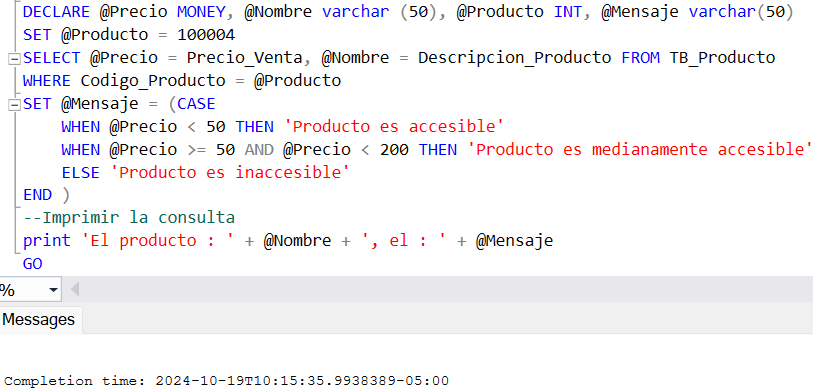
\includegraphics[scale = 0.5]{Imagenes/probs_resueltos/pr7.png}
  \caption{Problema resuelto 7}
\end{figure}

\subsection{Problema resuelto 8}

\begin{figure}[H]
  \centering
  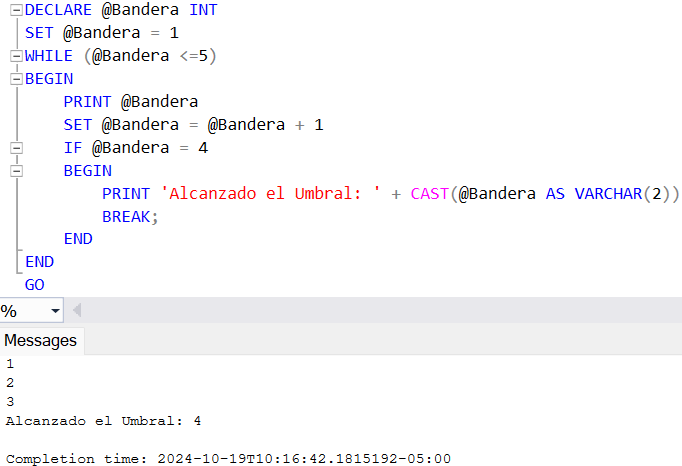
\includegraphics[scale = 0.5]{Imagenes/probs_resueltos/pr8.png}
  \caption{Problema resuelto 8}
\end{figure}

\subsection{Problema resuelto 9}

\begin{figure}[H]
  \centering
  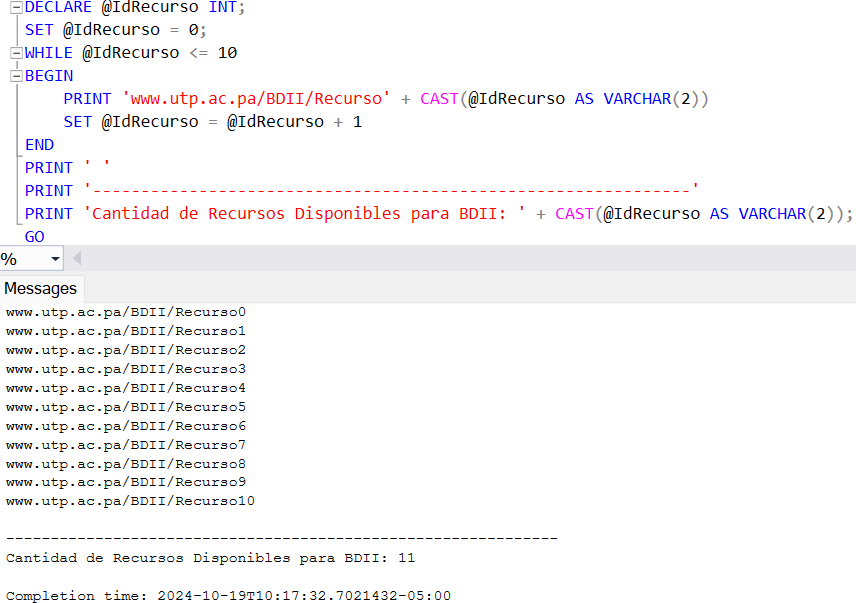
\includegraphics[scale = 0.5]{Imagenes/probs_resueltos/pr9.png}
  \caption{Problema resuelto 9}
\end{figure}

\subsection{Problema resuelto 10}

\begin{figure}[H]
  \centering
  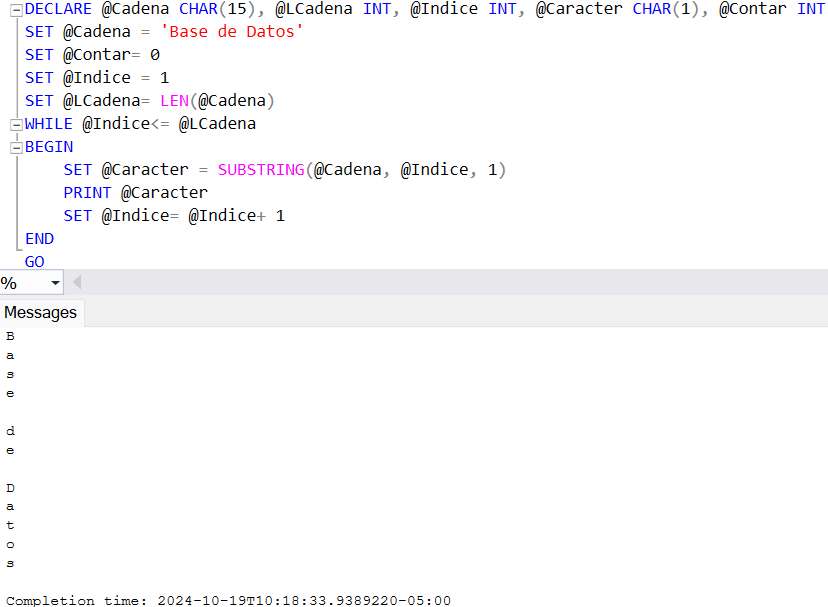
\includegraphics[scale = 0.5]{Imagenes/probs_resueltos/pr10.png}
  \caption{Problema resuelto 10}
\end{figure}

\subsection{Problema resuelto 11}

\begin{figure}[H]
  \centering
  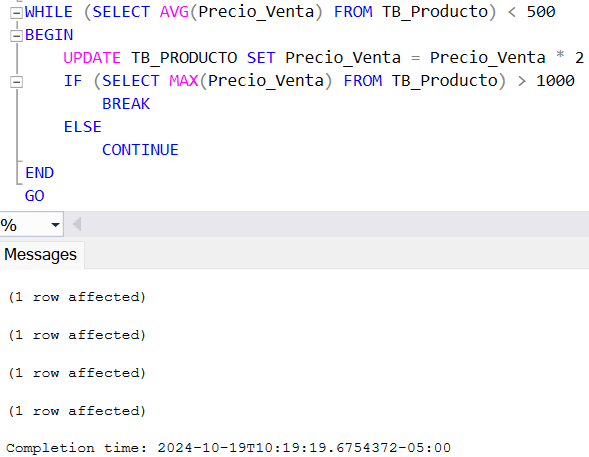
\includegraphics{Imagenes/probs_resueltos/pr11.png}
  \caption{Problema resuelto 11}
\end{figure}
\section{Problemas propuestos}
\subsection{Problema propuesto 1}

\begin{figure}[H]
  \centering
  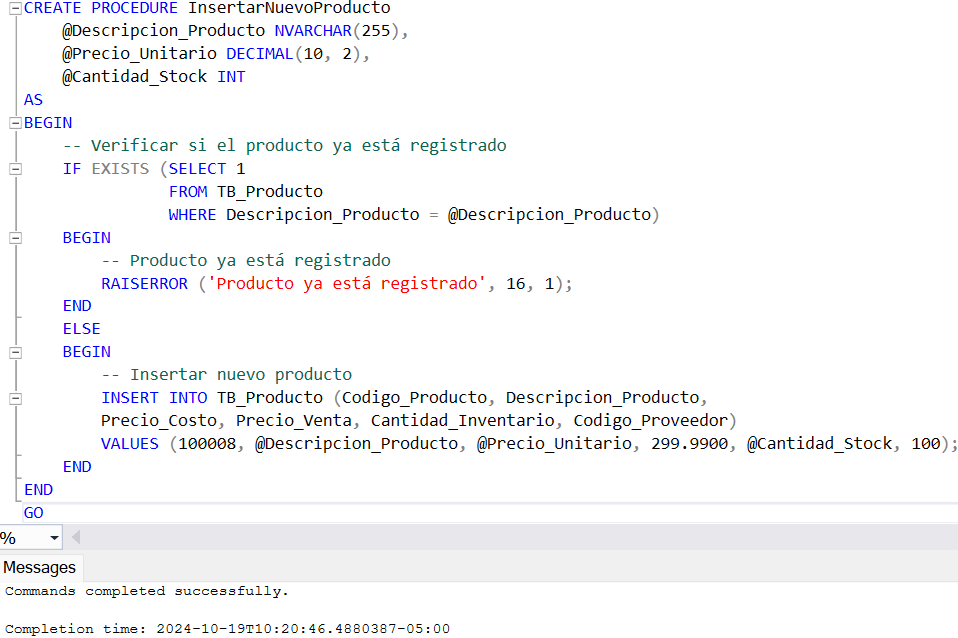
\includegraphics[scale = 0.5]{Imagenes/probs_propuestos/pp1.png}
  \caption{Problema propuesto 1}
\end{figure}

\begin{figure}[H]
  \centering
  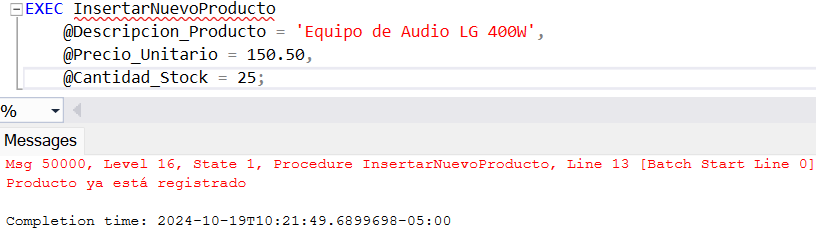
\includegraphics[scale = 0.5]{Imagenes/probs_propuestos/pp1_exe.png}
  \caption{Problema propuesto 1 ejecución}
\end{figure}

\subsection{Problema propuesto 2}

\begin{figure}[H]
  \centering
  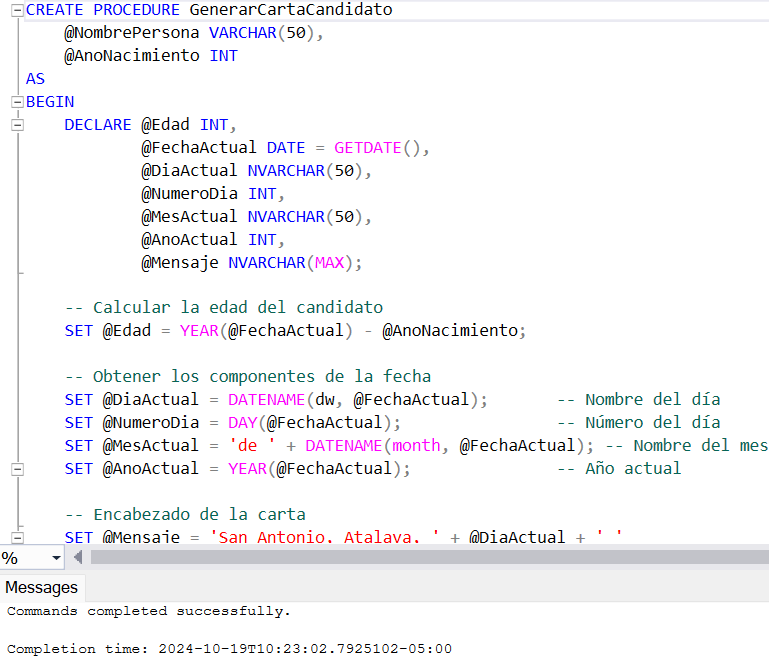
\includegraphics[scale = 0.5]{Imagenes/probs_propuestos/pp2.png}
  \caption{Problema propuesto 2}
\end{figure}

\begin{figure}[H]
  \centering
  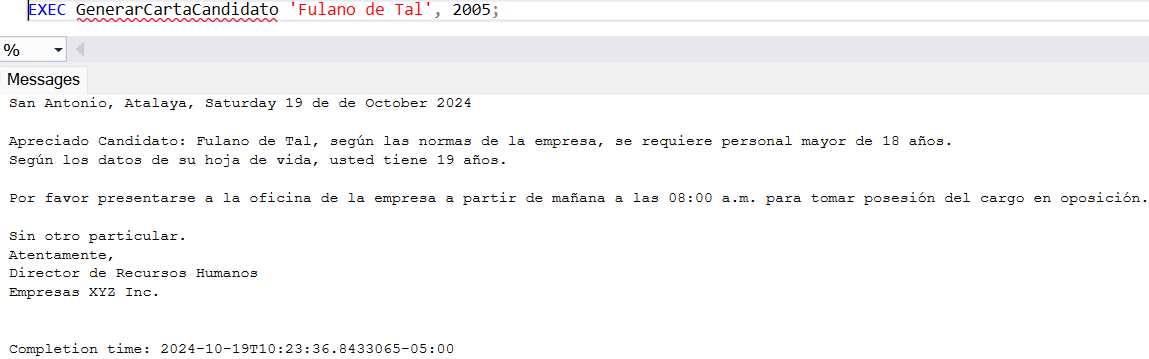
\includegraphics[scale = 0.5]{Imagenes/probs_propuestos/pp2_exe.png}
  \caption{Problema propuesto 2 ejecución}
\end{figure}

\subsection{Problema propuesto 3}

\begin{figure}[H]
  \centering
  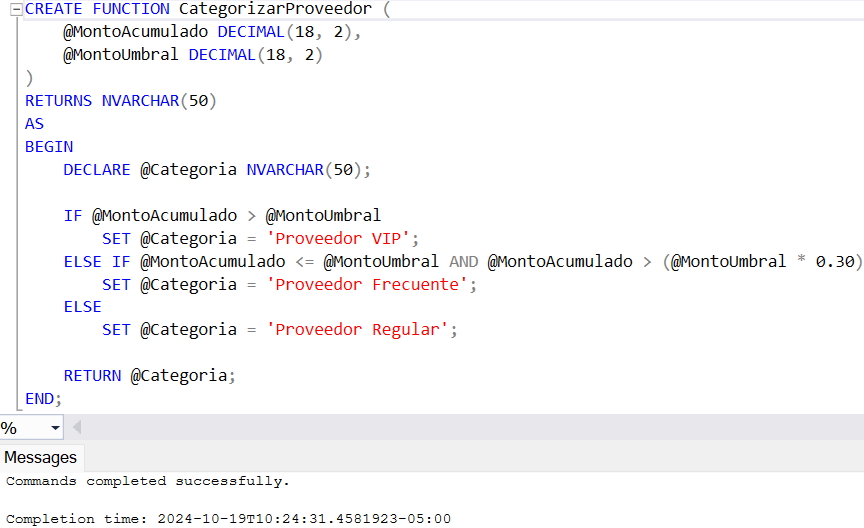
\includegraphics[scale = 0.5]{Imagenes/probs_propuestos/pp3.png}
  \caption{Problema propuesto 3}
\end{figure}

\begin{figure}[H]
  \centering
  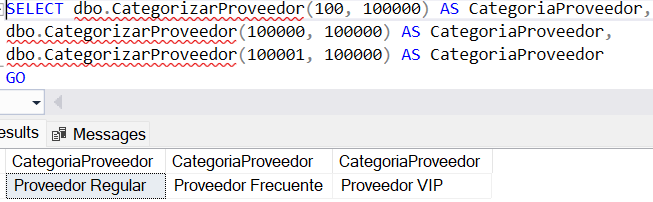
\includegraphics[scale = 0.5]{Imagenes/probs_propuestos/pp3_exe.png}
  \caption{Problema propuesto 3 ejecución}
\end{figure}

\subsection{Problema propuesto 4}

\begin{figure}[H]
  \centering
  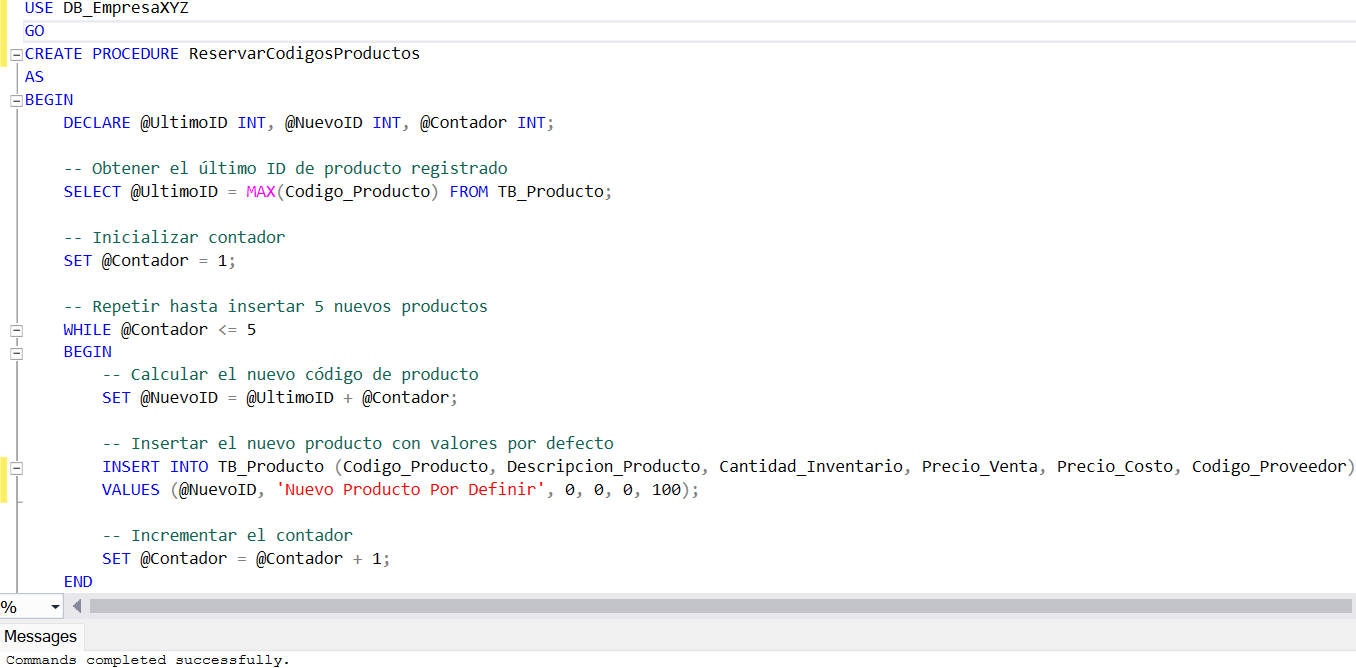
\includegraphics[scale = 0.4]{Imagenes/probs_propuestos/pp4.png}
  \caption{Problema propuesto 4}
\end{figure}

\begin{figure}[H]
  \centering
  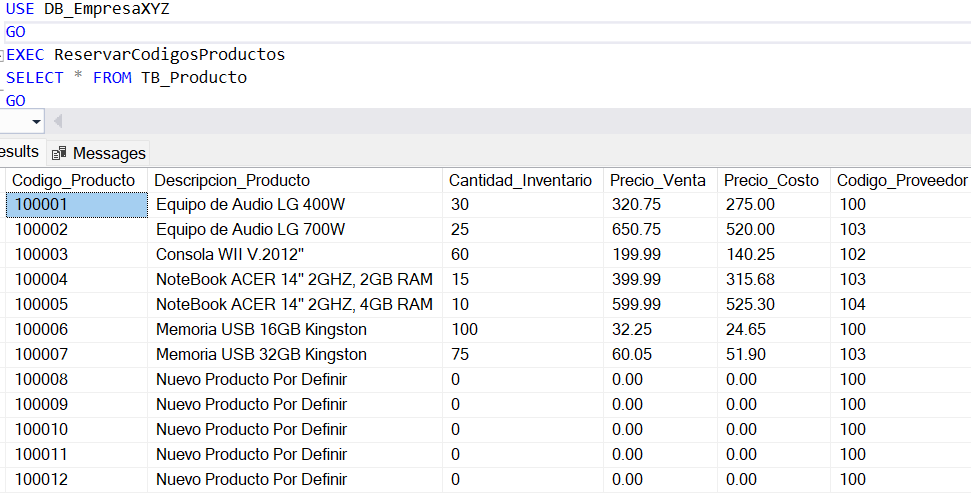
\includegraphics[scale = 0.5]{Imagenes/probs_propuestos/pp4_exe.png}
  \caption{Problema propuesto 4 ejecución}
\end{figure}
\end{document}